\section{Fonctionnement des failles}


Les deux failles utilisent le m\^eme principe et tiennent leur existence du fait que les anciennes versions des protocoles SSL/TLS comportent des failles. L'adversaire utilise une attaque de type "man in the middle" et force l'utilisation d'une version vulnérable de SSL, de manière à pouvoir exploiter ses failles. Parfois il n'est m\^eme pas utile de la forcer, car quand un navigateur doté d’une version récente n’arrive pas à se connecter à un serveur non mis à jour, ou mal configuré, il réessaie en utilisant des versions anciennes : c’est la downgrade dance, qui aboutit à l'utilisation d'une ancienne version vulnérable.

\subsection{Un point sur SSL/TLS}

\subsubsection{Historique}

SSL/TLS sont des protocoles qui fonctionnent suivant un mode client-serveur, et qui garantissent l'authentification du serveur et du client (optionnel), ainsi que la confidentialité et l'intégrité de données echangées. SSL est l'ancien nom de TLS, et a vécu sur 3 versions:
\begin{itemize}
\item 1994: SSL 1.0
\item Février 1995: SSL 2.0, première version réellement utilisée.
\item Novembre 1996: SSL 3.0 
\end{itemize}
TLS a ensuite pris le relais: 
\begin{itemize}
\item Janvier 1999: TLS 1.0
\item Avril 2006: TLS 1.1
\item Avril 2008: TLS 1.2
\end{itemize}
TLS, comme SSLv3, intègre un mécanisme de compatibilité ascendante avec les versions précédentes. Ainsi, quand le client et le serveur négocient la version du protocole qu'ils vont utiliser, ils peuvent choisir la plus récente commune aux deux. En Mars 2011, la compatibilité des versions TSL avec SSLv2 a été abandonnée. \\
La plupart des navigateurs supportent la version TSL 1.2:
\begin{itemize}
\item Google Chrome 30 et suivants
\item Mozilla Firefox 27 et suivants
\item Microsoft Internet Explorer 11 et suivants
\item Opera 17 et suivants
\item Apple Safari 7 et suivants
\end{itemize}
Plus précisément, TLS est composé de deux niveaux: TLS Record Protocol (couche transport) et TLS Handshake Protocol (couche session).

\subsubsection{TLS Handshake protocol}

Ce protocole permet l'authentification et l'échange de clés nécessaires pour établir une session sécurisée:
\begin{center}
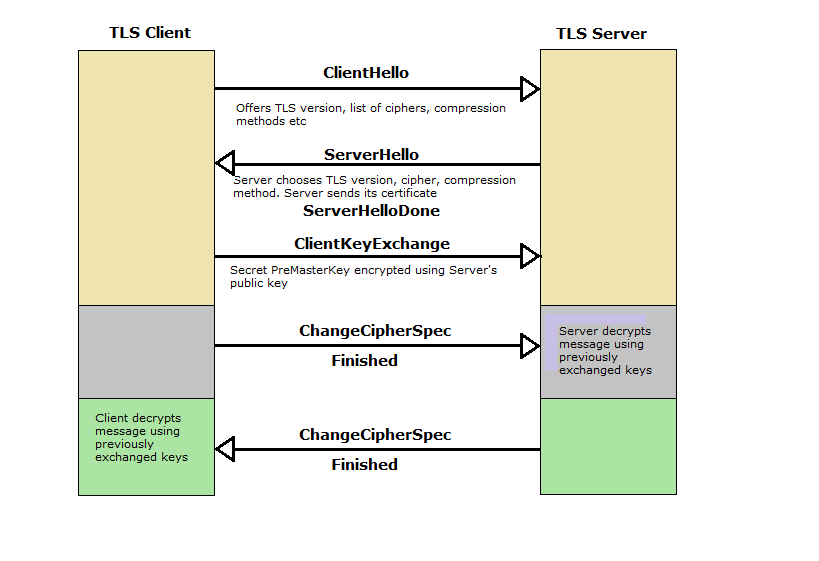
\includegraphics[scale=0.6]{img/tls-handshake.png}
\end{center}

Détails de chaque étape:
\begin{itemize}
\item le client envoie un message "ClientHello" au serveur, pour lui indiquer entre autres la dernière version TLS qu'il supporte, la liste des algorithmes de chiffrement qu'il supporte et les méthodes de compression qu'il supporte
\item le serveur renvoie un message "ServerHello", indiquant la version TLS, l'algorithme de chiffrement et la méthode de compression qui seront utilisés. Il envoie également son certificat (permettant l'authentification) et un nombre aléatoire
\item le serveur envoie un message "ServerHelloDone" pour indiquer qu'il a fini avec la première phase du handshake
\item le client génère un nombre appelé "PreMasterSecret", encrypté avec la clé publique du certificat du serveur
\item le client et le serveur génèrent alors leur secret partagé "Master Secret" à partir du nombre aléatoire et du "PreMasterSecret"
\item le client envoie un message "ChangeCipherSpec" indiquant que la suite de la communication sera cryptée, et envoie un message "Finished" qui est donc crypté
\item le serveur reçoit et décrypte le message et envoie son "ChangedCipherSpec"
\item le client reçoit et décrypte le message et c'est la fin du handshake
\end{itemize}
Les algorithmes utilisés pour l'échange de clés sont DH (Diffie-Hellman) et RSA.

\subsubsection{TLS Record Protocol}

Ce protocole permet de sécuriser les données en utilisant les clés qu'on a crée pendant le handshake. Il permet également de vérifier l'intégrité des données:
\begin{center}
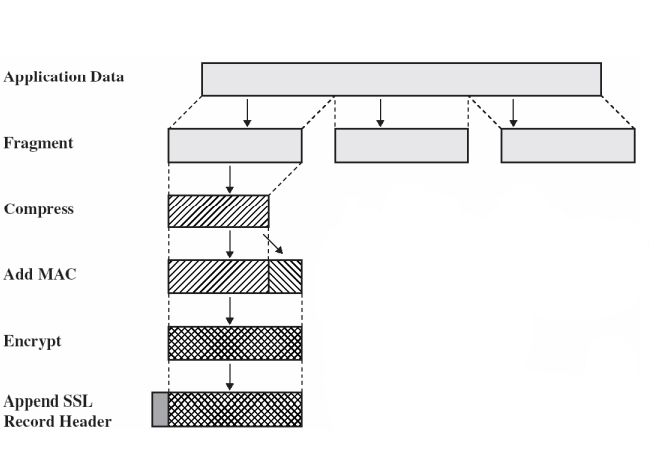
\includegraphics[scale=0.7]{img/tls-record.png}
\end{center}

Détails des étapes:
\begin{itemize}
\item on divise le message à transmettre en fragments 
\item on compresse les fragments
\item on applique MAC (message authentification code) pour authentifier les messages 
\item on crypte les messages
\item on ajoute un en-t\^ete
\end{itemize}
Une fois ceci réalisé, on passe à la couche suivante de transport (TCP). Quand on reçoit un message, on fait l'opération inverse (décryptage, vérification d'authenfication avec le MAC, décompression, défragmentation).


\subsection{La faille Poodle}

\subsection{La faille Freak}


